\documentclass[a4paper,10pt]{article}

\input{packages.tex}
\usetheme{metropolis}

\usepgfplotslibrary{dateplot}

\lstset{
  basicstyle=\ttfamily,
  mathescape
}

\title{Final}
\posttitle{\end{center}}

\begin{document}

\maketitle

\emergencystretch 3em

\input{recommendations.tex}

NOME: \rule{.85\textwidth}{0.1mm}

\begin{multicols*}{2}
\setlength{\leftmargini}{0pt}
\begin{enumerate}
  \item (2,0 pt) Use o princípio da indução para provar as afirmações a seguir.

  \begin{enumerate}
    \item (1,0 pt) $ 6^{n} + 4 $ é divisível por $ 5 $, para todo $ n \geq 0 $.
    \item (1,0 pt) $ 5^{2n+1} + 2^{2n+1} $ é divisível por $ 7 $, para todo $ n \geq 0 $.
  \end{enumerate}

  \item (1,5 pt) Considere o pseudocódigo abaixo:

  \begin{minted}{c}
Para i de 0 até n - 1:
  Para j de i + 1 até n - 1:
    Comando
  \end{minted}

    \begin{enumerate}
      \item (0,5 pt) Expresse como um somatório a quantidade de vezes que a linha \texttt{Comando} é executada.
      % \sum_{i = 0}^{n - 1} \sum_{j = i + 1}^{n - 1} 1
      \item (1,0 pt) Simplifique o somatório até chegar a uma fórmula em função de n. Para isso, use a expressão abaixo:
      \[
        \sum_{i = 0}^{n - 1} i = \frac{n(n - 1)}{2}
      \]
      % \frac{n(n - 1)}{2}
    \end{enumerate}

  \item (1,5 pt) Relacione cada complexidade de tempo com uma operação em um algoritmo.

  \begin{enumerate}
    \item $ O(n^2) $
    \item $ O(1) $
    \item $ O(n!) $
    \item $ O(\log{n}) $
    \item $ O(n) $
  \end{enumerate}

  \begin{enumerate}
    \item [(\textcolor{white}{c})] Percorrer um array do início ao fim
    \item [(\textcolor{white}{a})] Extrair de um array um elemento de índice x
    \item [(\textcolor{white}{d})] Percorrer uma matriz do início ao fim
    \item [(\textcolor{white}{e})] Gerar todas as permutações de um conjunto de dados
    \item [(\textcolor{white}{b})] Fazer uma busca binária em um array ordenado
  \end{enumerate}
  % (e)
  % (b)
  % (a)
  % (c)
  % (d)

  \vfill\null
  \columnbreak

  \item (1,8 pt) A imagem a seguir representa um \textit{grafo de Petersen}, com 10 vértices e 15 arestas. Faça uma BFS no grafo, começando a partir do vértice A e explorando em ordem alfabética. Desenhe a relação de parentesco do grafo no formato de árvore. Responda também se o grafo é bipartido ou não.
  % Fila: A B F I C J E G D H
  %  A  B  C  D  E  F  G  H  I  J
  % -1  A  B  I  F  A  F  I  A  B
  % Não é bipartido.

  \begin{center}
    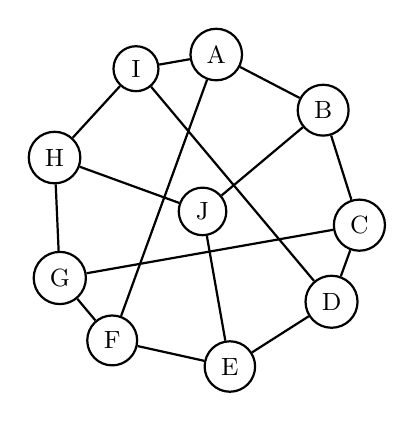
\begin{tikzpicture}[scale=0.5]
      \foreach \x\y in {1/A,4/D,7/G} {
        \node[circle, draw=black, thick] (\y) at ({-\x*40 + 125}:4){\small \y};
      }
      \foreach \x\y in {2/B,5/E,8/H} {
        \node[circle, draw=black, thick] (\y) at ({-\x*40 + 120}:4){\small \y};
      }
      \foreach \x\y in {3/C,6/F,9/I} {
        \node[circle, draw=black, thick] (\y) at ({-\x*40 + 115}:4){\small \y};
      }

      \node[circle, draw=black, thick] (J) at (0,0){\small J};

      \draw[thick]
        (A) -- (B) --
        (C) -- (D) --
        (E) -- (F) --
        (G) -- (H) --
        (I) -- (A);

      \draw[thick] (A) -- (F);
      \draw[thick] (I) -- (D);
      \draw[thick] (C) -- (G);
      \draw[thick] (J) -- (B);
      \draw[thick] (J) -- (H);
      \draw[thick] (J) -- (E);
    \end{tikzpicture}
  \end{center}

  \item (1,8 pt) Faça uma DFS no grafo a seguir, começando a partir do vértice A e explorando em ordem alfabética. Obtenha a relação de parentesco entre os vértices e desenhe essa relação no formato de uma árvore. Classifique todas as arestas do grafo.
  %  A  B  C  D  E  F  G
  % -1  A  B  C  C  C  B
  %
  % Arestas:
  % A - B Árvore
  % A - G Retorno
  % B - C Árvore
  % B - E Retorno
  % B - F Retorno
  % B - G Árvore
  % C - D Árvore
  % C - E Árvore
  % C - F Árvore

  \begin{center}
    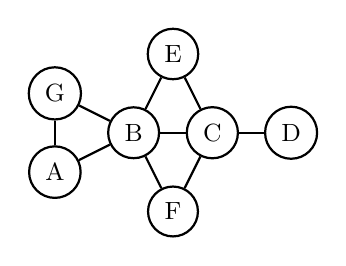
\begin{tikzpicture}
      \node[circle, draw=black, thick](A) at (0.00,-0.50){\small A};
      \node[circle, draw=black, thick](B) at (1.00, 0.00){\small B};
      \node[circle, draw=black, thick](C) at (2.00, 0.00){\small C};
      \node[circle, draw=black, thick](D) at (3.00, 0.00){\small D};
      \node[circle, draw=black, thick](E) at (1.50, 1.00){\small E};
      \node[circle, draw=black, thick](F) at (1.50,-1.00){\small F};
      \node[circle, draw=black, thick](G) at (0.00, 0.50){\small G};

      \draw[thick] (A) -- (G);
      \draw[thick] (A) -- (B);
      \draw[thick] (B) -- (G);
      \draw[thick] (B) -- (C);
      \draw[thick] (B) -- (E);
      \draw[thick] (B) -- (F);
      \draw[thick] (C) -- (E);
      \draw[thick] (C) -- (F);
      \draw[thick] (C) -- (D);
    \end{tikzpicture}
  \end{center}

  \item (1,4 pt) Encontre a árvore geradora mínima do grafo a seguir usando o algoritmo de Kruskal. Escreva a ordenação das arestas usada no algoritmo. Ordene as arestas que possuem o mesmo peso usando a ordem alfabética (lembre-se de ordenar as duas letras que definem as arestas em ordem alfabética também).
  % A - B 1 X
  % D - F 1 X
  % B - F 2 X
  % C - D 2 X
  % B - C 3
  % D - E 3 X
  % B - D 4
  % C - E 4
  % E - F 5
  % A - C 6
  % C - F 7

  \begin{center}
    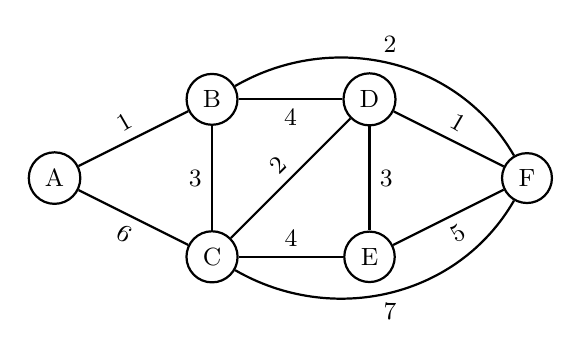
\begin{tikzpicture}
      \node[circle, draw=black, thick](A) at (0.00, 0.00){\small A};
      \node[circle, draw=black, thick](B) at (2.00, 1.00){\small B};
      \node[circle, draw=black, thick](C) at (2.00,-1.00){\small C};
      \node[circle, draw=black, thick](D) at (4.00, 1.00){\small D};
      \node[circle, draw=black, thick](E) at (4.00,-1.00){\small E};
      \node[circle, draw=black, thick](F) at (6.00, 0.00){\small F};

      \draw[thick] (A) -- node[rotate=30,anchor=south](){\small 1} (B);
      \draw[thick] (A) -- node[rotate=-30,anchor=north](){\small 6} (C);
      \draw[thick] (B) -- node[anchor=east](){\small 3} (C);
      \draw[thick] (B) -- node[anchor=north](){\small 4} (D);
      \draw[thick] (B) to [out= 30,in= 120] node[anchor=south](){\small 2} (F);
      \draw[thick] (C) -- node[rotate=45,anchor=south](){\small 2} (D);
      \draw[thick] (C) -- node[anchor=south](){\small 4} (E);
      \draw[thick] (C) to [out=-30,in=-120] node[anchor=north](){\small 7} (F);
      \draw[thick] (D) -- node[anchor=west](){\small 3} (E);
      \draw[thick] (D) -- node[rotate=-30,anchor=south](){\small 1} (F);
      \draw[thick] (E) -- node[rotate=30,anchor=north](){\small 5} (F);
    \end{tikzpicture}
  \end{center}
\end{enumerate}
\end{multicols*}
\end{document}
